\documentclass[11pt,letterpaper]{article}
\usepackage[T1]{fontenc}
\usepackage[scaled]{helvet}
\renewcommand{\familydefault}{\sfdefault}
\usepackage{amsmath,amssymb}
\usepackage[margin=0.8in,bottom=0.9in]{geometry}
\usepackage[most]{tcolorbox}
\usepackage{tikz}
\usetikzlibrary{calc}
\usepackage{enumitem}
\usepackage{array}
\usepackage{needspace}
\usepackage{fancyhdr}
\usepackage{pifont}

% ---- Palette "F. Bright & Playful" ----
\definecolor{fmtitle}{HTML}{3D2C8D}
\definecolor{fmkey}{HTML}{0096C7}
\definecolor{fmwatch}{HTML}{2BB673}
\definecolor{fmturn}{HTML}{F4A100}
\definecolor{fmmistake}{HTML}{EF476F}
\definecolor{fmnotice}{HTML}{9B5DE5}
\definecolor{fmgray}{HTML}{6B6B6B}

\pagestyle{fancy}
\fancyhf{}
\renewcommand{\headrulewidth}{0pt}
\fancyfoot[C]{\footnotesize\color{fmgray}\textcopyright\ 2026 FangMath. All rights reserved.}
\fancyfoot[R]{\footnotesize\color{fmgray}\thepage}
\setlength{\parindent}{0pt}
\setlength{\parskip}{3pt}

\newcommand{\badge}[1]{\colorbox{fmtitle}{\color{white}\bfseries\small\ #1\ }}
\newcommand{\leveltag}[2]{\colorbox{#1}{\color{white}\bfseries\scriptsize\ #2\ }}
\newcommand{\LE}{\leveltag{fmwatch}{EASY}}
\newcommand{\LM}{\leveltag{fmturn}{MEDIUM}}
\newcommand{\LH}{\leveltag{fmmistake}{HARD}}

\newcommand{\sectionbar}[2]{\needspace{6cm}\par\vspace{4mm}
  \begin{tcolorbox}[enhanced,colback=fmtitle,colframe=fmtitle,arc=2mm,
    left=4mm,top=1.5mm,bottom=1.5mm]
  \color{white}\bfseries\large #1\hfill{\normalsize\mdseries #2}
  \end{tcolorbox}}

\newtcolorbox{keyidea}{enhanced,breakable,colback=white,colframe=fmkey,boxrule=1pt,arc=2mm,
  title={Key Idea},coltitle=fmkey,fonttitle=\bfseries,
  attach boxed title to top left={xshift=4mm,yshift=-2mm},
  boxed title style={colback=white,colframe=fmkey,boxrule=0.9pt}}
\newtcolorbox{watchme}{enhanced,colback=white,colframe=fmwatch,boxrule=1pt,arc=2mm,
  title={Watch Me --- Worked Example},coltitle=fmwatch,fonttitle=\bfseries,
  attach boxed title to top left={xshift=4mm,yshift=-2mm},
  boxed title style={colback=white,colframe=fmwatch,boxrule=0.9pt}}
\newtcolorbox{mistakebox}{enhanced,breakable,colback=white,colframe=fmmistake,boxrule=1pt,arc=2mm,
  title={Common Mistake},coltitle=fmmistake,fonttitle=\bfseries,
  attach boxed title to top left={xshift=4mm,yshift=-2mm},
  boxed title style={colback=white,colframe=fmmistake,boxrule=0.9pt}}
\newtcolorbox{yourturn}{enhanced,breakable,colback=white,colframe=fmturn,boxrule=1pt,arc=2mm,
  title={Your Turn},coltitle=fmturn,fonttitle=\bfseries,
  attach boxed title to top left={xshift=4mm,yshift=-2mm},
  boxed title style={colback=white,colframe=fmturn,boxrule=0.9pt}}
\newtcolorbox{answerbox}[1]{enhanced,breakable,colback=white,colframe=fmwatch,boxrule=1pt,arc=2mm,
  title={#1},coltitle=fmwatch,fonttitle=\bfseries,
  attach boxed title to top left={xshift=4mm,yshift=-2mm},
  boxed title style={colback=white,colframe=fmwatch,boxrule=0.9pt}}

\newcommand{\work}[1]{\par\vspace{#1}}
\setlist[enumerate]{itemsep=2pt,topsep=3pt}

% ---------------- extra boxes ----------------
\newtcolorbox{notebox}{enhanced,breakable,colback=white,colframe=fmnotice,boxrule=1pt,arc=2mm,
  title={Notice},coltitle=fmnotice,fonttitle=\bfseries,
  attach boxed title to top left={xshift=4mm,yshift=-2mm},
  boxed title style={colback=white,colframe=fmnotice,boxrule=0.9pt}}
\newtcolorbox{exbox}{enhanced,colback=white,colframe=fmwatch,boxrule=0.8pt,arc=2mm,
  title={Example},coltitle=fmwatch,fonttitle=\bfseries\small,
  attach boxed title to top left={xshift=4mm,yshift=-2mm},
  boxed title style={colback=white,colframe=fmwatch,boxrule=0.8pt},fontupper=\small}
\newcommand{\topicbar}[1]{\needspace{4.5cm}\par\vspace{5mm}
  \begin{tcolorbox}[enhanced,colback=fmtitle,colframe=fmtitle,arc=2mm,left=4mm,top=1.5mm,bottom=1.5mm]
  \color{white}\bfseries\large #1
  \end{tcolorbox}}
\usepackage{multicol}

% ---------------- practice layout ----------------
\newcommand{\workline}{\par\vspace{7mm}{\color{gray!55}\rule{\linewidth}{0.4pt}}}
\newcommand{\worklines}[1]{\foreach \i in {1,...,#1}{\workline}}
\newcommand{\prob}[3]{\needspace{#3}\par\vspace{3mm}{\color{fmturn}\bfseries #1.}\ #2\par}
\newcommand{\ansline}{\par\vspace{4mm}\hfill\textbf{Answer:}\ \rule{5cm}{0.4pt}\par}
\newcommand{\keyitem}[3]{\needspace{3.2cm}\par\vspace{2mm}
  \begin{tcolorbox}[enhanced,colback=white,colframe=fmwatch!60,boxrule=0.6pt,arc=1.5mm,left=3mm,top=1.5mm,bottom=1.5mm]
  {\color{fmwatch}\bfseries #1.}\quad\small #2\par\vspace{1mm}
  \normalsize\textbf{Answer: #3}
  \end{tcolorbox}}



\newcommand{\grid}[1][0.32]{\begin{tikzpicture}[scale=#1]
 \draw[gray!30,thin] (-6,-6) grid (6,6);
 \draw[->,thick] (-6.4,0)--(6.5,0) node[right,font=\scriptsize]{$x$};
 \draw[->,thick] (0,-6.4)--(0,6.5) node[above,font=\scriptsize]{$y$};
 
\end{tikzpicture}}

\begin{document}
\colorbox{fmwatch}{\color{white}\bfseries\small\ ANSWER KEY\ }\hfill{\small\color{fmgray}Algebra 1 \textperiodcentered\ Systems of Equations}\par\vspace{4mm}
{\color{fmtitle}\LARGE\bfseries Systems of Linear Equations --- Answer Key}\par\vspace{1mm}

\needspace{4cm}\topicbar{Type 1 \quad Is It a Solution?}
\keyitem{1}{$2 + 3 = 5$ \ding{51}; \ $4 - 3 = 1$ \ding{51}}{Yes}
\keyitem{2}{$3 \cdot 1 + 1 = 4$ \ding{51}; \ $1 + 4 = 5 \neq 6$ \ding{55}}{No}
\keyitem{3}{$-2 + 6 = 4$ \ding{51}; \ $-2 \cdot (-1) = 2$ \ding{51}}{Yes}
\keyitem{4}{$3 - (-2) = 5$ \ding{51}; \ $3 + 2(-2) = -1 \neq 1$ \ding{55}}{No}
\needspace{4cm}\topicbar{Type 2 \quad Solve by Graphing}
\needspace{5.2cm}\par\vspace{2mm}\begin{tcolorbox}[enhanced,colback=white,colframe=fmwatch!60,boxrule=0.6pt,arc=1.5mm,left=3mm,top=1.5mm,bottom=1.5mm]\begin{minipage}[c]{0.58\linewidth}{\color{fmwatch}\bfseries 5.}\quad\small Graph both lines; they cross at $(2, 3)$. Check it in both equations.\par\vspace{1mm}\normalsize\textbf{Answer: $(2, 3)$}\end{minipage}\hfill\begin{minipage}[c]{0.38\linewidth}\centering 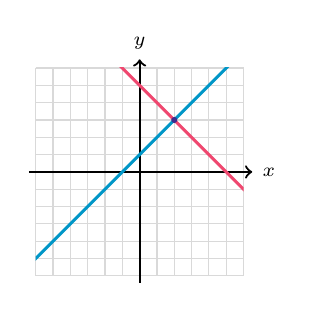
\begin{tikzpicture}[scale=0.22]
\draw[gray!30,thin] (-6,-6) grid (6,6);
\draw[->,thick] (-6.4,0)--(6.5,0) node[right,font=\scriptsize]{$x$};
\draw[->,thick] (0,-6.4)--(0,6.5) node[above,font=\scriptsize]{$y$};
\begin{scope}\clip (-6,-6) rectangle (6,6);
\draw[fmkey,line width=1.1pt] (-7,-6.000)--(7,8.000);
\draw[fmmistake,line width=1.1pt] (-7,12.000)--(7,-2.000);
\end{scope}
\fill[fmtitle] (2.0,3.0) circle (5pt);
\end{tikzpicture}\end{minipage}\end{tcolorbox}
\needspace{5.2cm}\par\vspace{2mm}\begin{tcolorbox}[enhanced,colback=white,colframe=fmwatch!60,boxrule=0.6pt,arc=1.5mm,left=3mm,top=1.5mm,bottom=1.5mm]\begin{minipage}[c]{0.58\linewidth}{\color{fmwatch}\bfseries 6.}\quad\small Graph both lines; they cross at $(4, 0)$. Check it in both equations.\par\vspace{1mm}\normalsize\textbf{Answer: $(4, 0)$}\end{minipage}\hfill\begin{minipage}[c]{0.38\linewidth}\centering 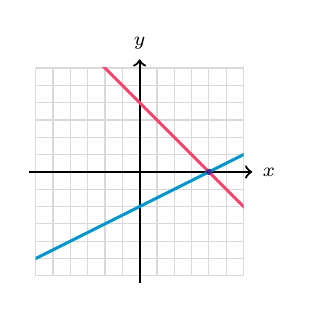
\begin{tikzpicture}[scale=0.22]
\draw[gray!30,thin] (-6,-6) grid (6,6);
\draw[->,thick] (-6.4,0)--(6.5,0) node[right,font=\scriptsize]{$x$};
\draw[->,thick] (0,-6.4)--(0,6.5) node[above,font=\scriptsize]{$y$};
\begin{scope}\clip (-6,-6) rectangle (6,6);
\draw[fmkey,line width=1.1pt] (-7,-5.500)--(7,1.500);
\draw[fmmistake,line width=1.1pt] (-7,11.000)--(7,-3.000);
\end{scope}
\fill[fmtitle] (4.0,0.0) circle (5pt);
\end{tikzpicture}\end{minipage}\end{tcolorbox}
\needspace{5.2cm}\par\vspace{2mm}\begin{tcolorbox}[enhanced,colback=white,colframe=fmwatch!60,boxrule=0.6pt,arc=1.5mm,left=3mm,top=1.5mm,bottom=1.5mm]\begin{minipage}[c]{0.58\linewidth}{\color{fmwatch}\bfseries 7.}\quad\small Graph both lines; they cross at $(2, 1)$. Check it in both equations.\par\vspace{1mm}\normalsize\textbf{Answer: $(2, 1)$}\end{minipage}\hfill\begin{minipage}[c]{0.38\linewidth}\centering 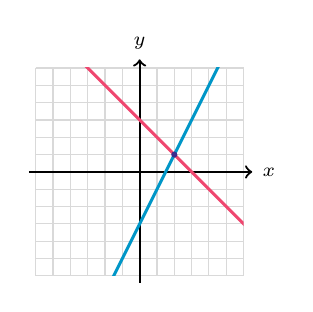
\begin{tikzpicture}[scale=0.22]
\draw[gray!30,thin] (-6,-6) grid (6,6);
\draw[->,thick] (-6.4,0)--(6.5,0) node[right,font=\scriptsize]{$x$};
\draw[->,thick] (0,-6.4)--(0,6.5) node[above,font=\scriptsize]{$y$};
\begin{scope}\clip (-6,-6) rectangle (6,6);
\draw[fmkey,line width=1.1pt] (-7,-17.000)--(7,11.000);
\draw[fmmistake,line width=1.1pt] (-7,10.000)--(7,-4.000);
\end{scope}
\fill[fmtitle] (2.0,1.0) circle (5pt);
\end{tikzpicture}\end{minipage}\end{tcolorbox}
\needspace{5.2cm}\par\vspace{2mm}\begin{tcolorbox}[enhanced,colback=white,colframe=fmwatch!60,boxrule=0.6pt,arc=1.5mm,left=3mm,top=1.5mm,bottom=1.5mm]\begin{minipage}[c]{0.58\linewidth}{\color{fmwatch}\bfseries 8.}\quad\small Graph both lines; they cross at $(2, -1)$. Check it in both equations.\par\vspace{1mm}\normalsize\textbf{Answer: $(2, -1)$}\end{minipage}\hfill\begin{minipage}[c]{0.38\linewidth}\centering 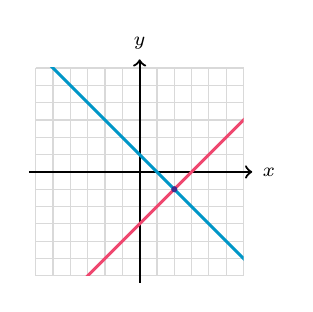
\begin{tikzpicture}[scale=0.22]
\draw[gray!30,thin] (-6,-6) grid (6,6);
\draw[->,thick] (-6.4,0)--(6.5,0) node[right,font=\scriptsize]{$x$};
\draw[->,thick] (0,-6.4)--(0,6.5) node[above,font=\scriptsize]{$y$};
\begin{scope}\clip (-6,-6) rectangle (6,6);
\draw[fmkey,line width=1.1pt] (-7,8.000)--(7,-6.000);
\draw[fmmistake,line width=1.1pt] (-7,-10.000)--(7,4.000);
\end{scope}
\fill[fmtitle] (2.0,-1.0) circle (5pt);
\end{tikzpicture}\end{minipage}\end{tcolorbox}
\needspace{4cm}\topicbar{Type 3 \quad Substitution}
\keyitem{9}{$x + 2x = 12$, \ $3x = 12$, \ $x = 4$; \ $y = 2 \cdot 4 = 8$}{$(4, 8)$}
\keyitem{10}{$2x + x + 3 = 9$, \ $3x = 6$, \ $x = 2$; \ $y = 5$}{$(2, 5)$}
\keyitem{11}{$3(y - 1) + y = 13$, \ $4y = 16$, \ $y = 4$; \ $x = 3$}{$(3, 4)$}
\keyitem{12}{$x - (-3x + 2) = 6$, \ $4x = 8$, \ $x = 2$; \ $y = -4$}{$(2, -4)$}
\keyitem{13}{$4x - 5 = 2x + 1$, \ $2x = 6$, \ $x = 3$; \ $y = 7$}{$(3, 7)$}
\keyitem{14}{$3y - 8 + 2y = 7$, \ $5y = 15$, \ $y = 3$; \ $x = 1$}{$(1, 3)$}
\needspace{4cm}\topicbar{Type 4 \quad Elimination}
\keyitem{15}{Add: $2x = 14$, \ $x = 7$; \ $y = 3$}{$(7, 3)$}
\keyitem{16}{Subtract: $4y = 12$, \ $y = 3$; \ $2x = 4$, \ $x = 2$}{$(2, 3)$}
\keyitem{17}{Add: $4x = 12$, \ $x = 3$; \ $y = 2$}{$(3, 2)$}
\keyitem{18}{Multiply the first by 2: $2x + 4y = 16$. Subtract: $x = 4$; \ $y = 2$}{$(4, 2)$}
\keyitem{19}{Multiply the first by 2: $4x + 2y = 14$. Add: $7x = 21$, \ $x = 3$; \ $y = 1$}{$(3, 1)$}
\keyitem{20}{Multiply the second by 3: $6x - 3y = 9$. Add: $10x = 10$, \ $x = 1$; \ $y = -1$}{$(1, -1)$}
\needspace{4cm}\topicbar{Type 5 \quad How Many Solutions?}
\keyitem{21}{Same slope 2, different $y$-intercepts: parallel lines.}{No solution}
\keyitem{22}{Different slopes (3 and $-1$): the lines cross once.}{One solution, $(2, 4)$}
\keyitem{23}{Divide the second by 2: $y = \tfrac12 x + 3$. Same line.}{Infinitely many}
\keyitem{24}{Same slope $-1$, different intercepts (5 and 9).}{No solution}
\keyitem{25}{The second is the first times 2: the same line.}{Infinitely many}
\keyitem{26}{Slopes $-4$ and 4 are different: one crossing, at $(0, 1)$.}{One solution, $(0, 1)$}
\needspace{4cm}\topicbar{Type 6 \quad Word Problems}
\keyitem{27}{$x + y = 20$, \ $x - y = 6$. Add: $2x = 26$.}{13 and 7}
\keyitem{28}{$c + w = 15$, \ $2c + 4w = 44$. \ $2c + 2w = 30$, subtract: $2w = 14$.}{8 chickens, 7 cows}
\keyitem{29}{$p + n = 10$, \ $2p + 3n = 24$. \ $2p + 2n = 20$, subtract: $n = 4$.}{4 notebooks (and 6 pens)}
\keyitem{30}{$C = 10m + 30$ and $C = 15m + 15$: \ $10m + 30 = 15m + 15$, \ $15 = 5m$.}{3 months, \$60}
\end{document}
